\cleardoublepage
% ==============================================================
\chapter{Discussion and outlook}
% ==============================================================

In the scope of this thesis, several software tools have been designed, 
developed and subsequently applied for the investigation of biological 
questions, including the quantitation program qTrace for the characterization 
of the chloroplast proteome of \cre~and its anaerobic response.
In addition, a re-designed version of the Genomic Peptide Finder was used
to establish an automated proteogenomic genome annotation pipeline.
These two systems have been implemented in the context of the data evaluation
platform Proteomatic.

\section{Decentralized MS/MS data evaluation infrastructure}

In order to facilitate software development and utilization, Proteomatic
was designed and implemented to provide a framework for the software
dealing with specific mass spectrometric questions that is presented in 
this thesis.
From the researcher's perspective, Proteomatic provides a way to create and
execute MS/MS data evaluation pipelines without the need to install each of
the individual software tools manually.
Every researcher with access to a computer is able to run data evaluation
pipelines of virtually arbritrary complexity in an independent fashion.
This independence is facilitated by the fact that the system runs on Windows,
Mac OS X, and Linux.
% ------------------------------------

\paragraph{Scalability and robustness.}

From the primary investigator's point of view, Proteomatic implements a 
decentralized data evaluation system, in which the data evaluation requirements
of every researcher can be typically accomodated for with a single computer,
resulting in optimal scalability of the system because each computer acts 
independently.
Furthermore, a distributed system as provided by Proteomatic results in 
increased robustness towards component failure and the lab-wide throughput
is not greatly diminished by one or two failing computers.
Due to the automatic software downloading and update features, a fully 
functional environment can be quickly restored on a new hardware unit.
% ------------------------------------
Therefore, Proteomatic provides an advantage in terms of system reliability 
over existing alternatives such as the Trans-Proteomics Pipeline (TPP) and 
The OpenMS Proteomics Pipeline (TOPP).
Although these systems provide more comprehensive functionality than Proteomatic
currently does, the setup and preparation of these systems to a point where
they become fully functional from the user's perspective is a time-consuming 
process.
Proteomatic is downloads and unpacks software automatically when it is required.
In addition, Proteomatic can be set up in such a way that all processing steps
are automatically tracked by a central server.
In the case that the file tracking server fails and cannot be reached, 
Proteomatic stores all reports which could not be sent locally and attempts
to re-send them the next time a script finishes.
Although the file tracking step is not crucial for data evaluation itself,


TPP requires the installation of an Apache web server for the purpose
of providing a web browser-based graphical user interface (GUI).
While the GUI is helpful for users, the required Apache web server presents a 
non-negligible security risk because it potentially renders the user's computer 
accessible from the Internet.
It can be expected that most users will be unaware of this issue and therefore
not take care to update the web server software regularly.
This issue is especially precarious on Windows and Mac OS X which do not 
natively provide centralized, automatic software updating.
Finally, because Proteomatic is easy to install, it is also beneficial in 
education, giving students the opportunity to gain hands-on MS/MS data 
evalution experience.

\paragraph{Rapid deployment of novel functionality.}

The fact that mass spectrometric data acquisition is constantly improving in
terms of quantity and quality has fueled the development of software tools for
various data evaluation-related purposes.
Most of these programs can be easily integrated into Proteomatic.
In addition, the deployment of novel, in-house developed functionality is
greatly facilitated by Proteomatic due to its support for multiple scripting
languages and the central script update mechanism.
When novel functionality is being developed, initial decisions should be made 
carefully.
Although Proteomatic can support virtually any programming language, it should
be noted that the choice of an appropriate language must be made carefully.
For example, choosing a programming language which exclusively runs on Windows,
such as C\# restricts the target audience and compromises further possibilities.
Using Proteomatic, tool developers can concentrate on the actual data 
processing and do not have to spend time on creating graphical user interfaces.
An example regarding the calculation of peptide masses is shown in 
Fig.~\ref{fig:rapid-development}.
This approach enables a data processing method development style to which the
`release early, release often' paradigm can be easily applied to 
\citep{Raymond2001}.
While this approach has the potential disadvantage of erroneous software
being deployed to users, especially in the early stages, the faster progress
achieved through early user feedback can be expected to improve the software
quickly.
Because Proteomatic provides a means to push software updates to users,
this approach is especially feasible.

\begin{figure}
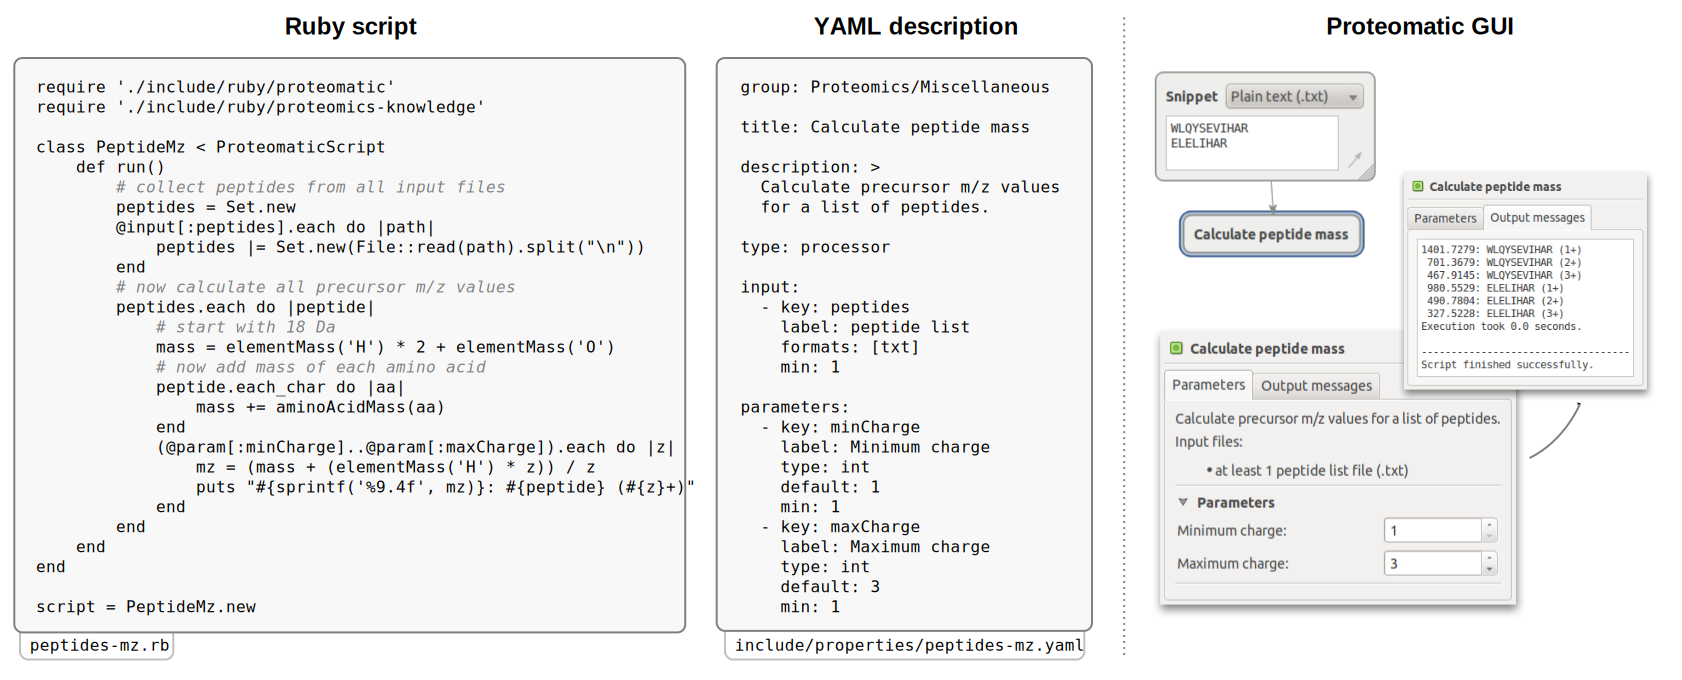
\includegraphics[width=\textwidth]{figures/example-script-2.jpg}
\caption{
{\bf An example of a Proteomatic script.} 
The script, which is implemented in Ruby in this case, is complemented with
a YAML-formatted description which specifies all parameters as well as input
and output files of the script.
The description is used by the Proteomatic front end to automatically construct 
a graphical user interface. This way, prototypes providing novel functionality
or proof of concepts can be deployed early and often.
}
\label{fig:rapid-development}
\end{figure}

\paragraph{File-based data processing.}

One might criticize the apparent lack of visualization capabilities in 
Proteomatic for experimental data and data evaluation results.
This is, however, a design decision which has been made to avoid {\em feature 
creep}, an effect which may lead to failure of software projects due to
an ever-increasing amount of features being implemented which go far beyond the 
originally intended scope.
Proteomatic implements a strictly file-based data processing pipeline which
means that all processing steps are strictly atomic and the output of one
processing step is passed on as one or several files.
This approach allows for manual inspection and intervention at any stage of
a complex pipeline.
Furthermore, all intermediate and final results can be copied to another 
computer or sent via e-mail.
Various standards are emerging for spectral data (mzML, \cite{Deutsch2008}), 
identification results (mzIdentML\footnote{http://www.psidev.info/index.php?q=node/319}), and quantitation results 
(mzQuantML\footnote{http://www.proteomexchange.org/project-organization/workpackages/wp2-standards-development}).
In addition to these standardized file formats, further established file 
formats such as plain text or comma-separated values are used for intermediate 
results.
For each of the file formats employed, specialized viewers already exist
or are currently in development\footnote{http://code.google.com/p/mzidentml-viewer}.
When the user double-clicks on an output file, Proteomatic delegates the
file handling to the underlying operating system which even has a program 
registered to handle the file type or may make a suggestion.
Therefore, a requirement for handling various file types within Proteomatic
is not evident.


% \begin{todo}
% - decentralized system
% - many researches, many computers for data evaluation
% - low impact of failing single computers on overall performance 
% - functional data evaluation setup can be restored in a straightforward way
% - automatic software downloading
% - also beneficial in education
% - two-level design (CLI and GUI) allows for usage in situations which too 
%   complex to be feasible for handling in the GUI
% - rapid deployment of novel functionality
% - support for multiple scripting languages
% 
% outlook:
% - remote execution and the cloud
% - filetracker queries


\section{Automated quantitation of metabolically labeled samples}

One of the studies presented in this thesis provides a comprehensive list of 
experimentally deduced chloroplast proteins for \cre~for the first time
(manuscript 2).
The list of 895 chloroplast-localized proteins has been compiled using
a quantitative approach via spectral counting.
The necessary data evaluation and filtering steps have been implemented
as processing steps in Proteomatic.
In manuscript 3, the list of chloroplast proteins has been manually extended 
to 996 proteins, including chloroplast-encoded proteins and further proteins
which have previously been characterized as localized to the chloroplast.
In addition to experimental localization, the anaerobic response of the 
experimentally deduced chloroplast proteome of the green alga is characterized 
in manuscript 2. 
From 895 proteins, 425 proteins could be quantified, confirming the anaerobic 
induction of hydrogenase, a protein involved in hydrogen production.
Furthermore, various proteins previously found to be induced on the transcript
level under anaerobiosis were also found induced in the protein sample.

The framework for high-throughput quantitation of metabolically labeled 
samples, in this case by SILAC, is provided by qTrace.
qTrace is a targeted quantitation program which takes a list of peptides
identified via MS/MS, along with their retention time, as input and then 
reconstructs the corresponding isotope envelopes which are subsequently 
matched to the full scans (see Appendix A for a detailed description).
In comparison to MS/MS-based quantitation, this strategy allows for the
incorporation of a large set of data points during the final peptide ratio
estimation because peptides usually elute for a time span long enough to
show their precursor peaks in several successive full scans.
It is obvious that the assignment of precursor peaks in full scans is highly
ambiguous, given the fact that several distinct peptides can yield the
same {\em m/z} values and therefore, peptide identification is not possible
using intact peptide masses only.
In order to remove spurious precursor peak assignments, several filters are 
employed.

\paragraph{Confidence of peak assignments.}

The inherent ambiguity resulting from assigning precursor peaks in full scans
is compensated with the requirement of MS/MS identification in the same band
within a small retention time window of one minute.
The assumption made by such a {\em MS/MS requirement filter} is that once the
identity of a precursor peak has been established via MS/MS, this information
can be expected to remain true within a short time span.
Furthermore, if protein fractionation via SDS-PAGE has been employed, a filter
which determines for each protein the SDS-PAGE band it has been most abundantly
identified in via MS/MS and subsequently discards all quantitation events
from other bands, allowing for a user-defined tolerance, under the assumption
that peak assignments in atypical bands are potential artifacts.

While these filters allow to increase the confidence of quantitation results
by coupling them to the identification results in both retention time and
molecular weight dimensions, assignments of peptides to intact precursor
peaks remains a challenge.
Therefore, quantitation results stemming from the analysis of full scans
should be regarded to provide induced candidate proteins in a discovery-based
experiment and further validation by employing molecular biology techniques
is advisable.

\paragraph{Metabolic labeling strategies.}

\begin{figure}
\includegraphics[width=\textwidth]{figures/qtrace-diagram.jpg}
\caption{
{\bf Quantitation results for \textsuperscript{15}N labeled \cre~samples
    under iron deficiency.} 
    Isolated chloroplast proteins from \cre~cultures grown under 
    iron-deficient (\textsuperscript{14}N) and iron-sufficient
    (\textsuperscript{15}N) conditions were mixed and measured via
    GeLC-MS/MS, using five bands from the gel.
    Using Proteomatic, a set of 2,754 distinct peptides could be identified
    via OMSSA which were subsequently passed to qTrace. 
    After carrying out all filtering steps as described in manuscript 2
    and shifting the quantitation results to the protein level,
    a set of 59 proteins or protein groups could be quantified,
    including many light-harvesting proteins.
    Ratios correspond to \textsuperscript{14}N/\textsuperscript{15}N ratios,
    high values correspond to induction under iron deficiency.
    The data presented in this figure was provided by Ricarda H\"ohner.
}
\label{fig:qtrace-15n}
\end{figure}

qTrace supports a variety of metabolic labeling strategies by allowing the 
user to define a non-natural isotope distribution for every chemical element 
occuring in amino acids (hydrogen, carbon, nitrogen, oxygen, and sulfur).
In addition, these non-natural isotope distributions can be applied 
to a restricted set of amino acids.
Using the user-specified label definition, qTrace is able to handle a variety
of labeling strategies, including SILAC, \textsuperscript{15}N labeling (see 
Fig. \ref{fig:qtrace-15n}), or \textsuperscript{18}O labeling 
\citep{Miyagi2007}.
\textsuperscript{13}C Arg SILAC labeling typically introduces a mass shift
of 6 Da between two sister peptides if trypsin is used for enzymatic digestion
because at most one arginine residue is typically expected per peptide and
arginine contains 6 carbon atoms.
Quantitation results stemming from \textsuperscript{15}N labeled samples
can be regarded as more confident because the mass shift between sister peptides
depends on the amino acid composition.
This is because the label is introduced into every amino acid, and the number of
nitrogen atoms is varying between different amino acids.

\paragraph{Induction of unannotated proteins.}

The large-scale quantitation approach presented in manuscript 2 resulted
in a couple of proteins of unknown function shown to be induced under
anaerobiosis.
The quantitative results for these proteins hint towards a possible role
in response to the experimental condition.
Therefore, such proteins present interesting candidates for further research.

\section{Proteogenomic genome annotation}

In manuscript 4, a new version of the Genomic Peptide Finder is presented
which has been redesigned and implemented from scratch to add two important 
features:

\begin{enumerate}
\item {\bf Intron splits may occur within a single coding nucleotide triplet.}
This addition increases search sensitivity by considering a possible intron
split in three locations per nucleotide triplet instead of one.

\item {\bf Splice donor/acceptor site consensus sequences may be specified.} 
This modification increases search specificity because spliced peptides with
unusual splice donor/acceptor sites are omitted from the results.
\end{enumerate}

Most importantly, the search has been greatly accelerated due to the use
of a one-time pre-processing step in which an index of the genomic DNA sequence
to be used is created.
For \cre, this indexing step produces an index file of 2.4 GiB in about 15 
minutes.
This initial cost is later compensated during the search which performs
20 queries per second on average on commodity hardware, using commodity flash 
memory to store the index file for faster random access.

Apart from these technical improvements, a method for the automated validation 
of GPF candidate peptides, employing standard database search programs such as 
OMSSA was established.
This allows for statistically robust identification of GPF-deduced peptides
alongside gene model peptides.
Furthermore, an annotation pipeline was established in which resulting GPF
peptides are passed to AUGUSTUS, which performs an {\em ab initio} gene 
model prediction supplemented by various extrinsic hint sources including
GPF peptides.
It is therefore a major contribution of this thesis that an automated
proteogenomic annotation of the \cre~genome in which MS/MS data generated
for various unrelated purposes can be re-used for the generation of
extrinsic AUGUSTUS hints is available.

\begin{figure}
\includegraphics[width=0.8\textwidth]{figures/gpf-omssa.jpg}
\caption{
{\bf Validation of GPF candidate peptides via a target/decoy approach
    using previously established gene models.} 
    Statistical significance of identified GPF candidate peptides is 
    assessed by employing a target/decoy approach with existing gene models 
    which may be incomplete but can be expected to contain a high amount of 
    correct sequences.
    GPF peptides are also added to the candidate peptide pool, and the database
    search program (OMSSA) assigns the best match from the pool to each
    MS/MS spectrum, resulting in comparable E-values in between the two
    peptide sources.
    The final E-value threshold determination is performed under exclusive
    consideration of the gene model target and decoy peptides.
    The determined threshold is then applied to all peptide/spectral matches,
    including those to GPF peptides.
}
\label{fig:gpf-omssa}
\end{figure}

The presented pipeline for the generation of peptide hints for the purpose of
proteogenomic annotation is similar to the exon splice graph approach proposed
by \citeauthor{Tanner2007} in that it uses MS/MS scans as a source of candidate
peptides.
However, the GPF approach is less biased in comparison to the exon splice graph
approach because it does not require exon/intron prediction as a first step.
GPF candidate peptides are solely generated from MS/MS {\em de novo} sequencing
and subsequent mapping of the resulting peptides to the genome, using a 
user-defined maximum intron length and a set of possible splice donor/acceptor 
site consensus sequences.
This means that intron prediction is carried out on a per-peptide basis, and
all peptides are treated independently.
The actual validation of extrinsic hints and splice site detection is
carried out by AUGUSTUS in the final annotation step.
Moreover, the approach is highly flexible because no specialized database
search program is required because candidate peptides are inferred by GPF
and then passed down the evaluation pipeline alongside a protein database
(see Fig.~\ref{fig:gpf-omssa}).

% \paragraph{Improved GPF performace.}

Although a gene model protein database is used to estimate the FDR of peptide 
identifications, the final GPF-deduced peptides which are exported as
peptide hints do not originate from this database, although in the case
of \cre, a large portion of these gene model peptides could be 
independently confirmed via the combination of {\em de novo} sequencing and 
GPF (see manuscript 4).
The high amount of 53\% confirmed gene model peptides points to a improvement 
of sensitivity of the new GPF version.
One might argue that the use of {\em de novo} prediction, followed by
error-tolerant, intron-aware matching to a genomic sequence is prone to
produce large sets of similar peptides.
However, this is not the case.
The 10 peptides which are generated by PEAKS for every MS/MS scan are 
reduced to 3.4 peptides on average after employment of GPF.
Furthermore, as has been shown in manuscript 4, 97\% of all GPF-deduced 
peptides are incorporated into the final gene models by AUGUSTUS.
Because several other hint sources were available to AUGUSTUS and none of
these sources is trusted unconditionally, these numbers suggest a strong 
specificity of GPF peptides.

\section{Identification of novel targets}

A combination of qTrace and the Genomic Peptide Finder can produce especially
interesting results.
As shown in manuscript 4, the Genomic Peptide Finder can confirm a substantial
amount of gene model peptides.
In addition, previously unknown peptides may result from the analysis.
This is especially true for organisms which for which genome sequencing and
genome annotation are unavailable or are still in the early stages.
Mass spectrometric data stemming from such organisms can be expected to
yield a high amount of novel peptides.
These peptides can be passed to qTrace along with identified gene model 
peptides, possibly resulting in the identification of induced peptides which
are not part of a gene model.
If there is a peptide A stemming from already existing, possibly preliminary gene
models, and a peptide B which has been identified via GPF only, and both
are shown to be co-regulated via qTrace, it might be that the gene model
containg A must be modified to also include B, if B is in close proximity to A
on the genome (and the direction of the reading frames of A and B is equal).
Quantitative information, mapped to the genome, might also be useful to
support proteogenomic genome annotation because peptide clusters exhibiting 
similar regulation patterns might be part of the same gene.

\begin{todo}
qTrace confirms GPF results, especially with 15N labeling
GPF confirms qTrace results ?
\end{todo}

\section{Outlook}

\subsection{Proteomatic}

\paragraph{Remote execution.}

\paragraph{Incorporation of a freely available {\em de novo} sequencing software.}

\paragraph{Centrally maintained repository of data files.}

\paragraph{Refinement of workflow interaction metaphors.}

\subsection{qTrace}

\paragraph{Performance comparison to existing alternatives.}

\paragraph{Untargeted quantitation.}

\subsection{Genomic Peptide Finder}

\paragraph{Increased search sensitivity.}

% outlook:
% - also provide data, not just tools
% - remote execution (but local creation)
% - refinement of the workflow interaction metaphors (batches should be defined
%   per arrow, not per input file box)
% \end{todo}
